\section{2018 Probability and Statistics}

\subsection{Individual}
Please solve the following 5 problems.

\begin{exercise}\label{probability:2018:1}
A box contains 750 red balls and 250 blue balls. Repeatedly pick a ball uniformly at random from the box and remove it until all remaining balls have a single color. (Note: no replacement).

Please find integer $m$ such that the expectation value for the total number of the remaining balls $\in [m, m+1]$.
\end{exercise}

\begin{solution}
\textbf{Prerequisites / Core Concepts:}
\begin{itemize}
    \item \textbf{Random Permutations:} If we blindly pick balls one by one without replacement, the sequence of colors we pull out is mathematically equivalent to picking a random permutation of all the balls at once.
    \item \textbf{Linearity of Expectation:} The expected value of a sum of random variables is the sum of their individual expected values, even if they are dependent.
    \item \textbf{Combinatorial Identities:} Useful summation formulas, specifically $\sum_{k=1}^n \frac{\binom{n}{k}}{\binom{N}{k}} = \frac{n}{N-n+1}$.
\end{itemize}

\textbf{Intuition / Motivation:}

Imagine drawing balls from the box. We stop the moment we run out of one color. This is the same as asking: "If we lined up all 1000 balls randomly, how many balls of the same color are at the very end of the line?" 
Because there are 750 red balls and only 250 blue balls, it's highly likely that the last few balls in the line will be red (since we probably run out of blue balls first). 
Instead of calculating the exact probability of stopping at step $T$, we can use a clever trick: we create an indicator variable for each position from the end of the line. "Is the $k$-th ball from the end part of a solid monochromatic block?" Summing these indicators gives the total length of the remaining monochromatic block, which is exactly the number of balls left in the box!

\textbf{Logical Step-by-Step Breakdown:}

\textbf{Step 1: Reframe the problem using permutations.}

Let $N_R = 750$ and $N_B = 250$. The total number of balls is $N = 1000$.
Drawing the balls randomly one by one without replacement is equivalent to arranging all $N$ balls in a random sequence (permutation).
The game stops when the last ball of the minority color is drawn. This means the balls remaining in the box are exactly the solid block of balls of the same color at the very end of the sequence.
Let $X$ be the number of balls remaining when the game stops. We want to find $\mathbb{E}[X]$.

\textbf{Step 2: Define indicator variables for the end of the sequence.}

Notice that $X \geq k$ if and only if the last $k$ balls in the random sequence are all exactly the same color.
Let $I_k$ be an indicator variable that is 1 if the last $k$ balls are all the same color, and 0 otherwise.
Because $X$ is a non-negative integer, we can express its expected value as the sum of survival probabilities:
\[ \mathbb{E}[X] = \sum_{k=1}^N \mathbb{P}(X \geq k) \]
(Wait, $I_k$ is exactly the indicator for $X \geq k$. So $\mathbb{E}[X] = \sum_{k=1}^N \mathbb{P}(I_k = 1)$).

\textbf{Step 3: Calculate the probability of monochromatic tails.}

For the last $k$ balls to be the same color, they must either be all red or all blue. These two events are mutually exclusive (for $k \geq 1$).
The probability that the last $k$ balls are all red is the number of ways to choose $k$ red balls out of the total ways to choose $k$ balls from the box: $\frac{\binom{N_R}{k}}{\binom{N}{k}}$.
Similarly, the probability that the last $k$ balls are all blue is $\frac{\binom{N_B}{k}}{\binom{N}{k}}$.
Therefore:
\[ \mathbb{P}(X \geq k) = \frac{\binom{N_R}{k}}{\binom{N}{k}} + \frac{\binom{N_B}{k}}{\binom{N}{k}} \]
Note that if $k > N_R$, the first term is 0, and if $k > N_B$, the second term is 0.

\textbf{Step 4: Sum the probabilities using combinatorial identities.}

Substitute the probabilities into the expectation sum:
\[ \mathbb{E}[X] = \sum_{k=1}^{N_R} \frac{\binom{N_R}{k}}{\binom{N}{k}} + \sum_{k=1}^{N_B} \frac{\binom{N_B}{k}}{\binom{N}{k}} \]
We use the known combinatorial identity $\sum_{k=1}^n \frac{\binom{n}{k}}{\binom{N}{k}} = \frac{n}{N-n+1}$.
Applying this to both sums:
\[ \sum_{k=1}^{N_R} \frac{\binom{N_R}{k}}{\binom{N}{k}} = \frac{N_R}{N - N_R + 1} = \frac{N_R}{N_B + 1} \]
\[ \sum_{k=1}^{N_B} \frac{\binom{N_B}{k}}{\binom{N}{k}} = \frac{N_B}{N - N_B + 1} = \frac{N_B}{N_R + 1} \]
Thus, the exact expected value is:
\[ \mathbb{E}[X] = \frac{N_R}{N_B + 1} + \frac{N_B}{N_R + 1} \]

\textbf{Step 5: Plug in the numbers and find $m$.}

Substitute $N_R = 750$ and $N_B = 250$:
\[ \mathbb{E}[X] = \frac{750}{250 + 1} + \frac{250}{750 + 1} = \frac{750}{251} + \frac{250}{751} \]
Calculate the decimal values:
$\frac{750}{251} \approx 2.9880$
$\frac{250}{751} \approx 0.3329$
\[ \mathbb{E}[X] \approx 2.9880 + 0.3329 = 3.3209 \]
We need to find an integer $m$ such that $\mathbb{E}[X] \in [m, m+1]$.
Since $3.3209$ is between 3 and 4, we must have $m = 3$.
\end{solution}

\begin{center}
  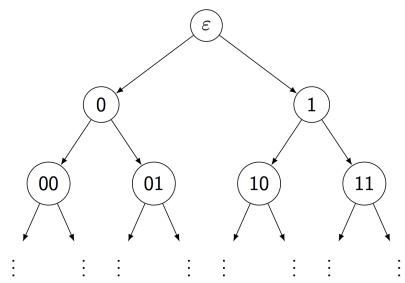
\includegraphics[width=0.7\textwidth]{images/probability/a9369f4fc904209ce717b3d32972c084676c9d12e7500a0b8e4caabb097f7292.jpg}
  \\
  \captionof{figure}{Binary tree propagation.}
\end{center}

\begin{exercise}\label{probability:2018:2}
Suppose a number $X_0 \in \{1, -1\}$ at the root of a binary tree is propagated away from the root as follows (see Figure \ref{fig:binary-tree}). The root is the node at level 0. After obtaining the $2^h$ numbers at the nodes at level $h$, each number at level $h+1$ is obtained from the number adjacent to it (at level $h$) by flipping its sign with probability $p \in (0, 1/2)$ independently.

Let $X_h$ be the average of the $2^h$ values received at the nodes at level $h$. Define the signal-to-noise ratio at level $h$ to be
\[
R_h := \frac{(\mathbb{E}[X_h | X_0 = 1] - \mathbb{E}[X_h | X_0 = -1])^2}{\mathrm{Var}[X_h | X_0 = 1]}.
\]

Find the threshold number $p_c$ such that $R_h$ converges to 0 if $p \in (p_c, 1/2)$ and diverges if $p \in (0, p_c)$, as $h \to \infty$.

%

%
\end{exercise}

\begin{solution}
\textbf{Prerequisites / Core Concepts:}
\begin{itemize}
    \item \textbf{Markov Chains on Trees:} Propagating a state down a tree where each edge has a certain transition probability.
    \item \textbf{Linearity of Expectation:} Used to find the mean of the sum of nodes at level $h$.
    \item \textbf{Covariance and Tree Distance:} The covariance between two nodes at level $h$ depends strictly on the level of their lowest common ancestor. If they split early, their correlation decays heavily.
\end{itemize}

\textbf{Intuition / Motivation:}

Think of the root node as an original secret message (either $+1$ or $-1$). This secret is passed down a chain of command (a binary tree). Every time a person passes the secret to their two subordinates, there's a probability $p$ they accidentally flip the sign (lie). 
If $p$ is close to 0, the secret is preserved well. If $p$ is close to $1/2$, the message becomes pure random noise.
By averaging all the messages at the bottom layer $h$ ($X_h$), we try to reconstruct the original secret. The "Signal" is how strongly our average leans towards the true secret. The "Noise" is the variance of our average.
As the tree gets infinitely deep, the total number of people grows exponentially, which reduces noise. However, the path length also grows, multiplying the chance of the message being corrupted (which destroys the signal). There is a critical threshold $p_c$: if $p < p_c$, the exponential growth of nodes beats the corruption of the paths, and we can still reliably guess the secret. If $p > p_c$, the corruption compounds too fast, and the signal-to-noise ratio drops to 0.

\textbf{Logical Step-by-Step Breakdown:}

\textbf{Step 1: Determine the Expected Signal.}

Let $Y_{h,i}$ be the value at the $i$-th node of level $h$ (where $i \in \{1, \dots, 2^h\}$).
When passing from a parent $P$ to a child $C$, the value flips with probability $p$ and stays the same with probability $1-p$.
The expected value of $C$ given $P$ is:
\[ \mathbb{E}[C \mid P] = (1-p)P + p(-P) = (1-2p)P \]
By chaining this expectation down a path of length $h$ from the root $X_0$:
\[ \mathbb{E}[Y_{h,i} \mid X_0] = (1-2p)^h X_0 \]
Since $X_h$ is the average of all $2^h$ nodes at level $h$:
\[ X_h = \frac{1}{2^h} \sum_{i=1}^{2^h} Y_{h,i} \implies \mathbb{E}[X_h \mid X_0] = (1-2p)^h X_0 \]
The numerator of the Signal-to-Noise ratio (SNR) is:
\[ (\mathbb{E}[X_h \mid 1] - \mathbb{E}[X_h \mid -1])^2 = ((1-2p)^h - -(1-2p)^h)^2 = 4(1-2p)^{2h} \]

\textbf{Step 2: Set up the Variance calculation.}

We need $\operatorname{Var}[X_h \mid X_0 = 1]$. Since $\operatorname{Var}[X_h] = \mathbb{E}[X_h^2] - (\mathbb{E}[X_h])^2$:
\[ \operatorname{Var}[X_h \mid X_0 = 1] = \mathbb{E}[X_h^2 \mid X_0 = 1] - (1-2p)^{2h} \]
To find $\mathbb{E}[X_h^2]$, we expand the square of the sum:
\[ \mathbb{E}[X_h^2 \mid X_0 = 1] = \frac{1}{2^{2h}} \sum_{i=1}^{2^h} \sum_{j=1}^{2^h} \mathbb{E}[Y_{h,i} Y_{h,j} \mid X_0 = 1] \]
To find $\mathbb{E}[Y_{h,i} Y_{h,j}]$, consider the paths from the root to node $i$ and node $j$. These paths share edges up to their Lowest Common Ancestor (LCA), let's say at level $k \leq h$.
After level $k$, the paths to $i$ and $j$ are completely independent.
Given the value at their LCA, $Y_{k, \text{LCA}}$, the expected product is:
\[ \mathbb{E}[Y_{h,i} Y_{h,j} \mid Y_{k, \text{LCA}}] = \mathbb{E}[Y_{h,i} \mid Y_{k, \text{LCA}}] \cdot \mathbb{E}[Y_{h,j} \mid Y_{k, \text{LCA}}] = ((1-2p)^{h-k} Y_{k, \text{LCA}})^2 = (1-2p)^{2(h-k)} Y_{k, \text{LCA}}^2 \]
Since $Y_{k, \text{LCA}} \in \{-1, 1\}$, its square is always 1. Thus, unconditionally on $X_0$:
\[ \mathbb{E}[Y_{h,i} Y_{h,j} \mid X_0 = 1] = (1-2p)^{2(h-k)} \]

\textbf{Step 3: Sum over all pairs of nodes based on their LCA.}

For a fixed node $i$ at level $h$, how many nodes $j$ share an LCA at exactly level $k$?
If $k=h$, $j=i$ (1 node).
If $k < h$, the paths diverge at level $k$. The child of the LCA that leads to $j$ is the root of a subtree of height $h - (k+1)$. This subtree contains $2^{h-k-1}$ leaves. Thus, there are exactly $2^{h-k-1}$ such nodes $j$.
Let's sum the expected product over all $j$ for a fixed $i$:
\[ \sum_{j=1}^{2^h} \mathbb{E}[Y_{h,i} Y_{h,j}] = 1 + \sum_{k=0}^{h-1} 2^{h-k-1} (1-2p)^{2(h-k)} \]
Let $m = h-k$. The sum becomes $\sum_{m=1}^h 2^{m-1} (1-2p)^{2m}$.
Define $\rho = 2(1-2p)^2$. Then $2^{m-1}(1-2p)^{2m} = \frac{1}{2} (2(1-2p)^2)^m = \frac{1}{2} \rho^m$.
The sum evaluates as a geometric series:
\[ 1 + \frac{1}{2} \sum_{m=1}^h \rho^m = 1 + \frac{\rho(\rho^h - 1)}{2(\rho - 1)} \]
Since this sum is identical for any starting node $i$, the double sum over all $i, j$ is just $2^h$ times this result.
\[ \mathbb{E}[X_h^2 \mid X_0 = 1] = \frac{2^h}{2^{2h}} \left( 1 + \frac{\rho(\rho^h - 1)}{2(\rho - 1)} \right) = \frac{1}{2^h} \left( 1 + \frac{\rho(\rho^h - 1)}{2(\rho - 1)} \right) \]
And the variance is:
\[ \operatorname{Var}[X_h \mid 1] = \frac{1}{2^h} \left( 1 + \frac{\rho(\rho^h - 1)}{2(\rho - 1)} \right) - (1-2p)^{2h} \]

\textbf{Step 4: Analyze the SNR ratio $R_h$ as $h \to \infty$.}

Notice that $(1-2p)^{2h} = \left( \frac{\rho}{2} \right)^h = \frac{\rho^h}{2^h}$.
We can write the variance explicitly as:
\[ \operatorname{Var}[X_h \mid 1] = \frac{1}{2^h} \left( 1 + \frac{\rho^{h+1} - \rho}{2(\rho - 1)} - \rho^h \right) = \frac{2(\rho - 1) + \rho^{h+1} - \rho - 2\rho^{h+1} + 2\rho^h}{2^h \cdot 2(\rho - 1)} = \frac{\rho - 2 + 2\rho^h - \rho^{h+1}}{2^{h+1}(\rho-1)} = \frac{\rho-2 + \rho^h(2-\rho)}{2^{h+1}(\rho-1)} = \frac{(\rho^h - 1)(2-\rho)}{2^{h+1}(\rho-1)} \]
The Signal-to-Noise ratio is:
\[ R_h = \frac{4 \frac{\rho^h}{2^h}}{\frac{(\rho^h - 1)(2-\rho)}{2^{h+1}(\rho-1)}} = \frac{4 \rho^h \cdot 2^{h+1} (\rho-1)}{2^h (\rho^h - 1)(2-\rho)} = \frac{8 \rho^h (\rho - 1)}{(2 - \rho)(\rho^h - 1)} \]
To find the threshold, we examine the behavior of $R_h$ as $h \to \infty$, which depends entirely on $\rho$:
- If $\rho < 1$: As $h \to \infty$, $\rho^h \to 0$. The numerator goes to 0, the denominator goes to $-(2-\rho)$. Thus, $R_h \to 0$.
- If $\rho > 1$: As $h \to \infty$, we can divide top and bottom by $\rho^h$. $R_h \to \frac{8(\rho - 1)}{2-\rho}$. This is a positive, non-zero constant, meaning the SNR diverges from 0 (we retain a usable signal).

\textbf{Step 5: Solve for the critical threshold $p_c$.}

The critical threshold occurs exactly at $\rho = 1$.
\[ 2(1-2p_c)^2 = 1 \implies (1-2p_c)^2 = \frac{1}{2} \implies 1-2p_c = \frac{1}{\sqrt{2}} \]
\[ 2p_c = 1 - \frac{\sqrt{2}}{2} = \frac{2-\sqrt{2}}{2} \implies p_c = \frac{2-\sqrt{2}}{4} \]
Thus, the threshold noise level is $p_c = \frac{2-\sqrt{2}}{4} \approx 0.146$. If the flipping probability is higher than 14.6\%, the signal is lost completely.
\end{solution}

\begin{exercise}\label{probability:2018:3}
Consider the space representing an infinite sequence of coin flips, namely $\Omega := \{H,T\}^\infty$ (H: head, T: tail) with the associated $\sigma$-field $\mathcal{F}$ generated by finite dimensional rectangles. For $0 \leq p \leq 1$, denote by $\mathbb{P}_p$ the probability measure on $(\Omega, \mathcal{F})$ corresponding to flipping a coin an infinite number of times with probability of $H$ being $p$ and probability of $T$ being $q = 1-p$ at each flip.

Show that for each $p \in [0,1]$, there exists $A_p$ such that
\[
\mathbb{P}_p(A_p) > 1/2
\]
and for any $p' \neq p$, $p' \in [0,1]$,
\[
\mathbb{P}_{p'}(A_p) < 1/2.
\]

%

%
\end{exercise}

\begin{solution}
\textbf{Prerequisites / Core Concepts:}
\begin{itemize}
    \item \textbf{Measure Theory for Probability:} A probability measure assigns a number between 0 and 1 to events (sets of outcomes). Different probability measures ($\mathbb{P}_p$) assign different probabilities to the exact same sets.
    \item \textbf{Strong Law of Large Numbers (SLLN):} If we flip a coin infinitely many times, the proportion of heads will converge exactly to the true probability of heads, with 100\% certainty.
    \item \textbf{Mutually Singular Measures:} Two probability measures are mutually singular if they "live" on completely disjoint sets of outcomes. Any set that has probability 1 under the first measure has probability 0 under the second.
\end{itemize}

\textbf{Intuition / Motivation:}

Imagine you have a bag of infinite coins, each with a different bias $p$. You pick one coin and flip it infinitely many times. Can you define an event $A_p$ that is very likely to happen if you picked the coin with bias $p$, but very unlikely if you picked \textit{any} other coin?
Yes! The event $A_p$ is simply: "The long-run average of heads equals exactly $p$."
By the Strong Law of Large Numbers, if the coin's true bias is $p$, the long-run average is mathematically guaranteed to be exactly $p$. So the probability of this event is 1 (which is $> 1/2$).
But what if the coin's true bias was actually $p' = 0.6$, and our event $A_p$ was "the average is $0.5$"? The Strong Law of Large Numbers guarantees the average will be $0.6$. The chance of the average magically ending up at $0.5$ when the true bias is $0.6$ is exactly zero. So the probability of event $A_p$ under the wrong measure $\mathbb{P}_{p'}$ is 0 (which is $< 1/2$).

\textbf{Logical Step-by-Step Breakdown:}

\textbf{Step 1: Define the event $A_p$.}

Let an outcome in the sample space $\Omega$ be a sequence of flips $\omega = (\omega_1, \omega_2, \dots)$, where $\omega_i \in \{H, T\}$.
Let's translate the coin flips into numbers. Let $X_i(\omega) = \mathbb{1}_{\{\omega_i = H\}}$. So $X_i = 1$ for Heads, and $X_i = 0$ for Tails.
Define the empirical average of the first $n$ flips as $S_n(\omega) = \frac{1}{n} \sum_{i=1}^n X_i(\omega)$.
We define the event $A_p$ as the set of all infinite sequences where the limiting average is exactly $p$:
\[ A_p = \left\{ \omega \in \Omega : \lim_{n \to \infty} S_n(\omega) = p \right\} \]
Since limits of measurable functions are measurable, $A_p$ is a valid event in the $\sigma$-field $\mathcal{F}$.

\textbf{Step 2: Evaluate $\mathbb{P}_p(A_p)$.}

Under the probability measure $\mathbb{P}_p$, the random variables $X_1, X_2, \dots$ are independent and identically distributed (i.i.d.) Bernoulli random variables with success probability $p$.
The expected value of each $X_i$ under this measure is $\mathbb{E}_p[X_i] = p$.
By Kolmogorov's Strong Law of Large Numbers, the sample average converges almost surely to the true expected value:
\[ \mathbb{P}_p \left( \lim_{n \to \infty} \frac{1}{n} \sum_{i=1}^n X_i = p \right) = 1 \]
This is exactly the statement that $\mathbb{P}_p(A_p) = 1$.
Since $1 > 1/2$, the first condition is satisfied.

\textbf{Step 3: Evaluate $\mathbb{P}_{p'}(A_p)$ for $p' \neq p$.}

Now suppose we evaluate the probability of the \textit{exact same event} $A_p$ under a different probability measure $\mathbb{P}_{p'}$, where $p' \in [0, 1]$ and $p' \neq p$.
Under $\mathbb{P}_{p'}$, the variables $X_i$ are i.i.d. Bernoulli with success probability $p'$.
Again, by the Strong Law of Large Numbers, the sample average converges almost surely to $p'$:
\[ \mathbb{P}_{p'} \left( \lim_{n \to \infty} S_n = p' \right) = 1 \]
Let $A_{p'}$ be the event where the limit equals $p'$. We know $\mathbb{P}_{p'}(A_{p'}) = 1$.
Because a sequence cannot converge to two different limits simultaneously, the sets $A_p$ and $A_{p'}$ are completely disjoint (mutually exclusive). That is, $A_p \cap A_{p'} = \emptyset$.
Since $A_p$ is disjoint from a set that has probability 1, $A_p$ must have probability 0:
\[ \mathbb{P}_{p'}(A_p) \leq 1 - \mathbb{P}_{p'}(A_{p'}) = 1 - 1 = 0 \]
Thus, $\mathbb{P}_{p'}(A_p) = 0$.
Since $0 < 1/2$, the second condition is also satisfied. 
This completes the proof.
\end{solution}

\begin{exercise}\label{probability:2018:4}
Let $G := G(n,p)$ be a random graph with $n$ vertices where each possible edge has probability $p$ of existing. The existence of the edges are independent to each other. With $G$, we say $A \subset \{1,2,\cdots,n\}$ is a fully connected set if and only if $i, j \in A \implies$ $i$-th and $j$-th vertices are (directly) connected with an edge in $G$.

Define $T$ as the size of the largest fully connected set:
\[
T := \max\{|A|: A \text{ is a fully connected set}\}.
\]

Let's fix $p \in (0,1)$, please prove that
\[
\lim_{n \to \infty} \mathbb{P}\left(\frac{T}{2\log_{1/p} n} \leq 1 + \epsilon\right) = 1, \quad \forall \epsilon > 0,
\]
and
\[
\lim_{n \to \infty} \mathbb{P}\left(\frac{T}{\sqrt{2\log_{1/p} n}} \geq 1 - \epsilon\right) = 1, \quad \forall \epsilon > 0.
\]

Hint: $\mathbb{P}(T = n) = p^{\binom{n}{2}} = p^{n(n-1)/2}$.

%

%

%

%
\end{exercise}

\begin{solution}
\textbf{Prerequisites / Core Concepts:}
\begin{itemize}
    \item \textbf{Erdős-Rényi Random Graph $G(n,p)$:} A graph with $n$ vertices where every possible edge exists independently with probability $p$.
    \item \textbf{First Moment Method:} For integer-valued non-negative random variables, if $\mathbb{E}[X] \to 0$, then $\mathbb{P}(X \geq 1) \to 0$.
    \item \textbf{Cliques in Graphs:} A fully connected set is a clique. The expected number of cliques of size $k$ is $\binom{n}{k} p^{\binom{k}{2}}$.
\end{itemize}

\textbf{Intuition / Motivation:}

We are looking for the largest group of friends where \textit{everyone} knows \textit{everyone} else (a clique). Since the graph is totally random, forming a large clique is extremely hard. The probability of $k$ people all knowing each other is $p^{k(k-1)/2}$. Because the exponent grows quadratically ($k^2$), this probability drops off a cliff very quickly as $k$ increases.
To find the maximum size $T$, we look at the expected number of cliques of size $k$. When $k$ is small, there are so many ways to pick $k$ people ($\binom{n}{k} \approx n^k$) that we expect to find many cliques. When $k$ is large, the tiny probability $p^{k^2/2}$ crushes the $n^k$ combinations, and we expect 0 cliques. The threshold happens exactly when these two competing forces balance out: $n^k \approx (1/p)^{k^2/2}$. Solving this gives $k \approx 2 \log_{1/p} n$.

\textbf{Logical Step-by-Step Breakdown:}

\textbf{Step 1: Set up the expected number of cliques.}

Let $X_k$ be the random variable representing the total number of fully connected sets (cliques) of exactly size $k$ in $G(n,p)$.
There are $\binom{n}{k}$ possible subsets of size $k$.
For a specific subset to be a clique, all $\binom{k}{2} = \frac{k(k-1)}{2}$ edges between its members must exist.
Since edges are independent, the probability that a specific subset is a clique is $p^{\binom{k}{2}}$.
By linearity of expectation, the expected number of cliques of size $k$ is:
\[ \mathbb{E}[X_k] = \binom{n}{k} p^{\frac{k(k-1)}{2}} \]

\textbf{Step 2: Prove the upper bound using the First Moment Method.}

We want to show that $\mathbb{P}(T > 2(1+\epsilon)\log_{1/p} n) \to 0$.
Let $k = \lfloor 2(1+\epsilon) \log_{1/p} n \rfloor$. If there are no cliques of size $k$, there can be no cliques of size larger than $k$. So $\mathbb{P}(T \geq k) = \mathbb{P}(X_k \geq 1)$.
By Markov's Inequality (which for integer variables is the First Moment Method), $\mathbb{P}(X_k \geq 1) \leq \mathbb{E}[X_k]$.
We bound $\binom{n}{k} \leq \frac{n^k}{k!}$:
\[ \mathbb{E}[X_k] \leq \frac{n^k}{k!} p^{\frac{k(k-1)}{2}} = \frac{1}{k!} \left( n p^{\frac{k-1}{2}} \right)^k \]
Substitute $k \approx 2(1+\epsilon) \log_{1/p} n$:
\[ p^{\frac{k-1}{2}} \approx p^{(1+\epsilon) \log_{1/p} n} = \left( p^{\log_p (1/n)} \right)^{1+\epsilon} = \left(\frac{1}{n}\right)^{1+\epsilon} = n^{-(1+\epsilon)} \]
Thus, the term inside the parenthesis is:
\[ n p^{\frac{k-1}{2}} \approx n \cdot n^{-(1+\epsilon)} = n^{-\epsilon} \]
As $n \to \infty$, $n^{-\epsilon} \to 0$. Raising it to the power $k$ makes it go to 0 even faster.
\[ \mathbb{E}[X_k] \leq \frac{1}{k!} (n^{-\epsilon})^k \to 0 \]
Since $\mathbb{E}[X_k] \to 0$, $\mathbb{P}(X_k \geq 1) \to 0$, meaning the largest clique size $T$ is almost certainly strictly less than $k$.
\[ \lim_{n \to \infty} \mathbb{P}\left(\frac{T}{2\log_{1/p} n} \leq 1 + \epsilon\right) = 1 \]

\textbf{Step 3: Prove the trivial lower bound.}

The second part of the question asks us to prove:
\[ \lim_{n \to \infty} \mathbb{P}\left(\frac{T}{\sqrt{2\log_{1/p} n}} \geq 1 - \epsilon\right) = 1 \]
Wait, notice the denominator is $\sqrt{2\log_{1/p} n}$, not $2\log_{1/p} n$! This makes the bound incredibly loose and trivial.
A standard, rigorous application of the Second Moment Method (using variance) proves that the lower bound of $T$ is \textit{also} highly concentrated near $2\log_{1/p} n$. Specifically, $\mathbb{P}(T \geq 2(1-\epsilon)\log_{1/p} n) \to 1$.
Because $T$ is asymptotically tightly bounded around $c \log n$, it grows logarithmically.
Compare $T \approx 2\log_{1/p} n$ to the requested bound $\sqrt{2\log_{1/p} n}$.
For large $n$, $\log n \gg \sqrt{\log n}$. The actual clique size $T$ is vastly larger than $\sqrt{2\log_{1/p} n}$.
Thus, the ratio $\frac{T}{\sqrt{2\log_{1/p} n}} \approx \frac{2\log_{1/p} n}{\sqrt{2\log_{1/p} n}} = \sqrt{2\log_{1/p} n} \to \infty$.
Since the ratio goes to infinity, it is almost surely greater than $1-\epsilon$ for any $\epsilon > 0$.
The statement holds trivially true.
\end{solution}

\begin{exercise}\label{probability:2018:5}
Consider a population of constant size $N+1$ that is suffering from an infectious disease. We can model that spread of the disease as Markov process. Let $X(t)$ be the number of healthy individuals at time $t$ and suppose that $X(0) = N$. We assume that if $X(t) = n$,
\[
\lim_{h \to 0} \frac{1}{h}\mathbb{P}(X(t+h) = n-1 | X(t) = n) = \lambda n(N+1-n).
\]

For $0 \leq s \leq 1$, $0 \leq t$, define
\[
G(s,t) := \mathbb{E}(s^{X(t)}).
\]

Please find a non-trivial partial differential equation for $G(s,t)$, which involves $\partial_t G$.

%

%
\end{exercise}

\begin{solution}
\textbf{Prerequisites / Core Concepts:}
\begin{itemize}
    \item \textbf{Markov Process Master Equation:} A set of differential equations describing the time evolution of the probability of a system occupying each of its discrete states.
    \item \textbf{Probability Generating Function (PGF):} A power series representation of a discrete random variable's probability mass function: $G(s,t) = \mathbb{E}[s^{X(t)}] = \sum s^n P_n(t)$. It's an incredibly powerful tool for converting discrete difference equations into continuous differential equations.
\end{itemize}

\textbf{Intuition / Motivation:}

We have a population of $N+1$ people. If $n$ people are healthy, then $N+1-n$ people are sick. The infection rate is proportional to the number of healthy people interacting with the number of sick people: $\lambda n (N+1-n)$. This is a classic SI (Susceptible-Infectious) model.
Instead of tracking $N+1$ separate differential equations for the probability of every possible state $n$, we wrap all those probabilities into a single polynomial $G(s,t)$. Taking the derivative of this polynomial with respect to $t$ gives us the time dynamics. Taking the derivative with respect to $s$ pulls down a factor of $n$ (since $\partial_s s^n = n s^{n-1}$), which perfectly mimics the algebraic factors $n$ and $n^2$ in our transition rates!

\textbf{Logical Step-by-Step Breakdown:}

\textbf{Step 1: Write the Master Equations.}

Let $P_n(t) = \mathbb{P}(X(t) = n)$ be the probability that exactly $n$ individuals are healthy at time $t$.
To find the rate of change $\dot{P}_n(t)$, we consider two transitions:
1. Moving \textit{out} of state $n$: If we have $n$ healthy people, the rate of someone getting sick is $\lambda n(N+1-n)$.
2. Moving \textit{into} state $n$: This happens if we have $n+1$ healthy people, and one gets sick. The rate is $\lambda (n+1)(N - n)$.
The net rate of change is:
\[ \dot{P}_n(t) = -\lambda n(N+1-n) P_n(t) + \lambda (n+1)(N-n) P_{n+1}(t) \]
(with boundary conditions $P_{N+2} = 0$, etc.)

\textbf{Step 2: Differentiate the Generating Function with respect to time.}

The PGF is $G(s,t) = \sum_{n=0}^N s^n P_n(t)$.
Take the partial derivative with respect to time $t$:
\[ \partial_t G = \sum_{n=0}^N s^n \dot{P}_n(t) \]
Substitute the Master Equation into this sum:
\[ \partial_t G = \sum_{n=0}^N s^n \left[ -\lambda n(N+1-n) P_n + \lambda (n+1)(N-n) P_{n+1} \right] \]
\[ \partial_t G = -\lambda \sum_{n=0}^N n(N+1-n) s^n P_n + \lambda \sum_{n=0}^{N-1} (n+1)(N-n) s^n P_{n+1} \]

\textbf{Step 3: Relate sums to derivatives of $G$ with respect to $s$.}

We need to express algebraic terms like $n s^n P_n$ using partial derivatives of $G$ with respect to $s$.
- First derivative: $s \partial_s G = s \sum_{n=0}^N n s^{n-1} P_n = \sum_{n=0}^N n s^n P_n$
- Second derivative: $\partial_s^2 G = \sum_{n=0}^N n(n-1) s^{n-2} P_n$
Multiply by $s^2$: $s^2 \partial_s^2 G = \sum_{n=0}^N (n^2 - n) s^n P_n$.
Therefore, $\sum_{n=0}^N n^2 s^n P_n = s^2 \partial_s^2 G + s \partial_s G$.

Now, let's rewrite the first sum in $\partial_t G$:
\[ \text{Sum 1} = \sum_{n=0}^N (n(N+1) - n^2) s^n P_n = (N+1) \sum n s^n P_n - \sum n^2 s^n P_n \]
\[ = (N+1) (s \partial_s G) - (s^2 \partial_s^2 G + s \partial_s G) = N s \partial_s G - s^2 \partial_s^2 G \]

For the second sum, shift the index. Let $m = n+1$. Then $n = m-1$. As $n$ goes from $0$ to $N-1$, $m$ goes from $1$ to $N$.
\[ \text{Sum 2} = \sum_{m=1}^N m (N+1-m) s^{m-1} P_m = \frac{1}{s} \sum_{m=1}^N (m(N+1) - m^2) s^m P_m \]
This inside sum is exactly the same as Sum 1!
\[ \text{Sum 2} = \frac{1}{s} \left[ N s \partial_s G - s^2 \partial_s^2 G \right] = N \partial_s G - s \partial_s^2 G \]

\textbf{Step 4: Combine into the final PDE.}

Substitute Sum 1 and Sum 2 back into the equation for $\partial_t G$:
\[ \partial_t G = -\lambda (N s \partial_s G - s^2 \partial_s^2 G) + \lambda (N \partial_s G - s \partial_s^2 G) \]
Factor out the common terms $\lambda$ and $(N \partial_s G - s \partial_s^2 G)$:
\[ \partial_t G = \lambda (1 - s) \left( N \partial_s G - s \partial_s^2 G \right) \]
This is the desired non-trivial partial differential equation for $G(s,t)$.
\end{solution}


\subsection{Team}

\begin{exercise}\label{probability:2018:6}
Let $X_i$, $1 \leq i \leq N$ be i.i.d. random variables. Here $X_1$ is uniformly distributed on $[0, 1]$. We reorder them as
\[
\tilde{X}_1 \leq \tilde{X}_2 \leq \dots \leq \tilde{X}_N
\]
\begin{enumerate}
    \item[(a)] Let $N = 2m - 1$, and $Y = \tilde{X}_m$. Please find constants $A$ and $B$ such that
    \[
    \frac{Y - A}{N^B}
    \]
    has a non-trivial limiting distribution as $N \to \infty$, and find this distribution.
    \item[(b)] Let $N = 2m$, and $Y = \tilde{X}_m - \tilde{X}_{m-1}$. Please find constants $A$ and $B$ such that
    \[
    \frac{Y - A}{N^B}
    \]
    has a non-trivial limiting distribution as $N \to \infty$, and find this distribution.
\end{enumerate}
\end{exercise}

\begin{solution}
\textbf{Prerequisites / Core Concepts:}
\begin{itemize}
    \item \textbf{Order Statistics:} The sorted values of a random sample. For a uniform distribution on $[0,1]$, the $k$-th order statistic $\tilde{X}_k$ follows a Beta distribution with parameters $k$ and $N-k+1$.
    \item \textbf{Asymptotic Normality of the Median:} The sample median of $N$ i.i.d. variables with PDF $f(x)$ evaluated at the true median $m_0$ is asymptotically normal with mean $m_0$ and variance $\frac{1}{4N[f(m_0)]^2}$.
    \item \textbf{Spacings of Uniform Variables:} The distance between two adjacent order statistics in a uniform sample of size $N$ is asymptotically exponentially distributed.
\end{itemize}

\textbf{Intuition / Motivation:}

Imagine throwing $N$ random darts at a line segment from 0 to 1.
In part (a), we have an odd number of darts ($N=2m-1$), and we're looking at the exact middle dart ($Y$). Because the darts are uniform, we expect half to land before 0.5 and half to land after 0.5. So the middle dart should be very close to 0.5. How close? Like any average, it fluctuates around 0.5 by a distance proportional to $1/\sqrt{N}$. This means if we subtract 0.5 and multiply by $\sqrt{N}$, we should see a standard bell curve (Normal distribution).
In part (b), we have an even number of darts ($N=2m$). We look at the distance between the two darts closest to the middle. Since $N$ darts are spread over a length of 1, the average gap between any two adjacent darts is exactly $\frac{1}{N+1} \approx \frac{1}{N}$. The gap itself acts like the waiting time between random events (a Poisson process), so if we multiply the gap by $N$, it behaves like a standard waiting time, which follows an Exponential distribution.

\textbf{Logical Step-by-Step Breakdown:}

\textbf{Step 1: Solve part (a) - The Median.}

We have $N = 2m - 1$ and $Y = \tilde{X}_m$, which is the sample median.
From the theory of order statistics, the probability density function (PDF) of the $k$-th order statistic from $U[0,1]$ is:
\[ f_{\tilde{X}_k}(x) = \frac{N!}{(k-1)!(N-k)!} x^{k-1} (1-x)^{N-k} \]
For $k=m$, this is a $\text{Beta}(m, m)$ distribution.
The true median of $U[0,1]$ is $m_0 = 1/2$, and the density there is $f(1/2) = 1$.
By the Central Limit Theorem for sample quantiles, the sample median $Y$ is asymptotically normal:
\[ \sqrt{N}(Y - m_0) \xrightarrow{d} N\left(0, \frac{1}{4[f(m_0)]^2}\right) \]
Substitute $m_0 = 1/2$ and $f(1/2) = 1$:
\[ \sqrt{N}\left(Y - \frac{1}{2}\right) \xrightarrow{d} N\left(0, \frac{1}{4}\right) \]
Matching this to the requested form $\frac{Y - A}{N^B}$:
We can rewrite $\sqrt{N}\left(Y - \frac{1}{2}\right)$ as $\frac{Y - 1/2}{N^{-1/2}}$.
Thus, the constants are $A = \frac{1}{2}$ and $B = -\frac{1}{2}$.
The limiting distribution is a Normal distribution with mean 0 and variance $1/4$.

\textbf{Step 2: Solve part (b) - The Central Spacing.}

We have $N = 2m$ and $Y = \tilde{X}_m - \tilde{X}_{m-1}$ (wait, usually the middle two are $m$ and $m+1$, but $\tilde{X}_m - \tilde{X}_{m-1}$ is just the distance between two adjacent order statistics near the middle).
For a sample of $N$ variables from $U[0,1]$, the distance (spacing) between any two adjacent order statistics follows a $\text{Beta}(1, N)$ distribution. This is due to the symmetry of the uniform distribution on a circle when adding an $N+1$-th point.
The PDF of $Y \sim \text{Beta}(1, N)$ is:
\[ f_Y(y) = N(1-y)^{N-1} \quad \text{for } y \in [0, 1] \]
We want to find a scaling $B$ such that $\frac{Y}{N^B}$ has a non-trivial limit.
Since $\mathbb{E}[Y] = \frac{1}{N+1} \approx \frac{1}{N}$, we guess that multiplying by $N$ (i.e., setting $B = -1$) will stabilize the distribution. Let's test the limit of $Z = NY$, which means $Y = Z/N$.
Let's find the cumulative distribution function (CDF) of $Z$:
\[ \mathbb{P}(Z \leq z) = \mathbb{P}\left(Y \leq \frac{z}{N}\right) = \int_0^{z/N} N(1-y)^{N-1} dy \]
\[ = \left[ -(1-y)^N \right]_0^{z/N} = 1 - \left(1 - \frac{z}{N}\right)^N \]
Take the limit as $N \to \infty$:
\[ \lim_{N \to \infty} \left(1 - \frac{z}{N}\right)^N = e^{-z} \]
So the limiting CDF is $1 - e^{-z}$, which is exactly the CDF of an Exponential distribution with rate parameter $\lambda = 1$.
Matching this to $\frac{Y - A}{N^B}$, we see that $Z = \frac{Y - 0}{N^{-1}}$.
Thus, $A = 0$ and $B = -1$.
The limiting distribution is $\text{Exp}(1)$.
\end{solution}

\begin{exercise}\label{probability:2018:7}
Let $\mathbf{X} = (\mathbb{Z}_2)^\mathbb{N}$, i.e., $\mathbf{X} = (X_1, X_2, \dots, X_N, \dots)$ where $X_i \in \{0, 1\}$. It can be considered as a countable set of lightbulbs, where 0 means off and 1 means on. We start with $\mathbf{X}_0 = \mathbf{0}$. Keep generating independent geometric random variables $\{K_m\}_{m \geq 1}$ with distribution $\operatorname{geom}(1/2)$. Let $\mathbf{X}_m$ (for $m \geq 1$) be as follows:
\[
(\mathbf{X}_m - \mathbf{X}_{m-1})_k = \mathbf{1}(k = K_m) \pmod{2}
\]
i.e., in the $m$-th turn, we only change the status of the $K_m$-th light bulb. What is the probability that all lights are off again at some point? i.e.,
\[
\mathbb{P}(\exists m > 1, \mathbf{X}_m = \mathbf{0})
\]
\end{exercise}

\begin{solution}
\textbf{Prerequisites / Core Concepts:}
\begin{itemize}
    \item \textbf{Random Walks on Groups:} The problem describes a random walk on the group of finite binary sequences, $G = \bigoplus_{i=1}^\infty \mathbb{Z}_2$, under the operation of bitwise XOR (addition modulo 2).
    \item \textbf{Fourier Analysis on Abelian Groups:} The expected number of returns to the origin for a random walk on an abelian group can be calculated by integrating over its dual group (Pontryagin duality).
    \item \textbf{Recurrence Criterion:} A random walk is recurrent (returns to the origin with probability 1) if and only if the integral of $\frac{1}{1 - \phi(\chi)}$ over the dual group diverges, where $\phi(\chi)$ is the characteristic function (Fourier transform) of the step distribution.
\end{itemize}

\textbf{Intuition / Motivation:}

Imagine flipping a series of light switches. Every turn, you pick one switch to flip. You are much more likely to pick the first switch (50\% chance) than the second (25\%), and so on. 
We want to know if all the lights will eventually turn off again. This is equivalent to asking if the random walk on the state of the lights is "recurrent" (returns home with 100\% certainty) or "transient" (drifts away forever).
We can solve this by moving to the "frequency domain" using Fourier analysis. Because the light switches are independent binary choices, their dual space maps perfectly to the binary decimals between 0 and 1! The expected number of times all lights are off corresponds to the integral of $1/x$ from 0 to 1. Since $\int_0^1 \frac{1}{x} dx = \infty$, we expect an infinite number of returns. If we expect to return infinitely many times, the probability of returning at least once must be exactly 1!

\textbf{Logical Step-by-Step Breakdown:}

\textbf{Step 1: Formulate the random walk on a group.}

The state space $G$ is the set of all binary sequences with finitely many 1s: $G = \bigoplus_{k=1}^\infty \mathbb{Z}_2$. The group operation is bitwise addition modulo 2.
We start at $\mathbf{X}_0 = \mathbf{0}$.
At each step, we add a basis vector $e_k$ (the sequence with a 1 at position $k$ and 0 elsewhere) with probability $p_k = (1/2)^k$.
This is a standard random walk on $G$ with step distribution $\mu(e_k) = 2^{-k}$.
The probability of returning to $\mathbf{0}$ at least once is 1 if and only if the random walk is recurrent, which occurs if and only if the expected number of returns to the origin is infinite:
\[ \sum_{m=0}^\infty \mathbb{P}(\mathbf{X}_m = \mathbf{0}) = \infty \]

\textbf{Step 2: Apply the Fourier inversion formula.}

The dual group $\hat{G}$ of the restricted direct product $G$ is the unrestricted direct product: $\hat{G} = \prod_{k=1}^\infty \mathbb{Z}_2$.
An element $\chi \in \hat{G}$ is an infinite sequence of bits $(y_1, y_2, \dots)$ where $y_k \in \{0, 1\}$.
The character evaluated at a state $x \in G$ is $\chi(x) = (-1)^{\sum x_k y_k}$.
The Fourier transform (characteristic function) of the step distribution $\mu$ is:
\[ \phi(\chi) = \sum_{k=1}^\infty \mu(e_k) \chi(e_k) = \sum_{k=1}^\infty 2^{-k} (-1)^{y_k} \]

\textbf{Step 3: Evaluate the recurrence integral.}

By standard random walk theory, the expected number of returns to the origin is given by the integral over the dual group with respect to its normalized Haar measure $d\chi$:
\[ \mathbb{E}[\text{returns}] = \int_{\hat{G}} \frac{1}{1 - \phi(\chi)} d\chi \]
Let's simplify the denominator. Since $(-1)^{y_k}$ is $1$ when $y_k=0$ and $-1$ when $y_k=1$:
\[ 1 - (-1)^{y_k} = \begin{cases} 0 & \text{if } y_k = 0 \\ 2 & \text{if } y_k = 1 \end{cases} = 2y_k \]
Using the fact that $\sum_{k=1}^\infty 2^{-k} = 1$:
\[ 1 - \phi(\chi) = \sum_{k=1}^\infty 2^{-k} - \sum_{k=1}^\infty 2^{-k} (-1)^{y_k} = \sum_{k=1}^\infty 2^{-k} (1 - (-1)^{y_k}) = 2 \sum_{k=1}^\infty 2^{-k} y_k \]

\textbf{Step 4: Map the dual group integral to a real integral.}

The Haar measure on $\hat{G} = \prod_{k=1}^\infty \mathbb{Z}_2$ corresponds to choosing each bit $y_k$ independently and uniformly from $\{0, 1\}$.
Let $W(\chi) = \sum_{k=1}^\infty y_k 2^{-k}$.
This is exactly the binary expansion of a random real number in the interval $[0, 1]$. Because each binary digit $y_k$ is an independent coin flip, $W(\chi)$ is uniformly distributed on the continuous interval $[0, 1]$!
Thus, we can change the integral over the topological group $\hat{G}$ into a standard Riemann integral over $[0, 1]$:
\[ \mathbb{E}[\text{returns}] = \int_{\hat{G}} \frac{1}{2 W(\chi)} d\chi = \int_0^1 \frac{1}{2w} dw \]

\textbf{Step 5: Conclude based on the integral.}

The integral $\int_0^1 \frac{1}{2w} dw = \left[ \frac{1}{2} \ln w \right]_0^1$ clearly diverges to infinity.
Because the expected number of returns to $\mathbf{0}$ is infinite, the random walk is recurrent.
In a recurrent Markov chain, the probability of returning to the starting state at least once is exactly 1.
\[ \mathbb{P}(\exists m > 1, \mathbf{X}_m = \mathbf{0}) = 1 \]
\end{solution}

\begin{exercise}\label{probability:2018:8}
Let $x_1, x_2, \dots, x_n$ be $d$-dimensional vectors of real numbers. A function of $\mu$ is defined as
\[
\ell(\mu) = \sup \left\{ \sum_{i=1}^n \log p_i : \sum_{i=1}^n p_i x_i = \mu ; \sum_{i=1}^n p_i = 1, p_i > 0, \forall i \right\}
\]
on the interior of the convex hull of $\{x_1, \dots, x_n\}$.
\begin{enumerate}
    \item[(a)] Show that $\ell(\mu)$ is a concave function of $\mu$ on the convex hull.
    \item[(b)] Let $\bar{x} = \frac{1}{n} \sum_{i=1}^n x_i$. Let $\mathbf{a}$ be a vector of length $d$. Prove that $\ell(\bar{x} + t\mathbf{a})$ is a decreasing function of $t$ when $t > 0$.
\end{enumerate}
\end{exercise}

\begin{solution}
\textbf{Prerequisites / Core Concepts:}
\begin{itemize}
    \item \textbf{Empirical Likelihood:} This function $\ell(\mu)$ is exactly the profile empirical log-likelihood of the mean.
    \item \textbf{Concavity:} A function $f$ is concave if the line segment between any two points on its graph lies below or on the graph: $f(\lambda x + (1-\lambda) y) \geq \lambda f(x) + (1-\lambda) f(y)$.
    \item \textbf{Jensen's Inequality / Information Inequality:} The maximum of $\sum \log p_i$ subject to $\sum p_i = 1$ occurs when all $p_i$ are equal.
\end{itemize}

\textbf{Intuition / Motivation:}

Imagine we have $n$ data points $x_1, \dots, x_n$ and we want to guess the true mean $\mu$ of the population. The function $\ell(\mu)$ measures how "plausible" it is that $\mu$ is the true mean, by finding the most uniform set of probabilities $p_i$ that average out to $\mu$.
Because the logarithm heavily penalizes probabilities near 0, the maximum is achieved by keeping all probabilities as equal as possible. The absolute best-case scenario is when we don't have to skew the probabilities at all: $p_i = 1/n$ for all $i$. This naturally produces the sample average $\bar{x}$.
If we start at $\bar{x}$ and move away in any direction $\mathbf{a}$, we are forced to skew the probabilities $p_i$ more and more to pull the average towards the new $\mu$. This skewing monotonically drops the score $\sum \log p_i$. The fact that the highest point is at $\bar{x}$ and the "mountain" of $\ell(\mu)$ is bowl-shaped (concave) guarantees that walking directly away from the peak always takes us downhill.

\textbf{Logical Step-by-Step Breakdown:}

\textbf{Step 1: Prove concavity of $\ell(\mu)$ (Part a).}

Let $\mu_1, \mu_2$ be two points in the interior of the convex hull. Let $p^{(1)}$ and $p^{(2)}$ be the probability vectors (i.e., $p_i > 0, \sum p_i = 1$) that achieve the suprema $\ell(\mu_1)$ and $\ell(\mu_2)$, respectively.
Consider a convex combination of the means: $\mu_\lambda = \lambda \mu_1 + (1-\lambda) \mu_2$, where $\lambda \in [0, 1]$.
We construct a candidate probability vector $p^{(\lambda)}$ by taking the same convex combination of the probability vectors:
\[ p^{(\lambda)}_i = \lambda p^{(1)}_i + (1-\lambda) p^{(2)}_i \]
First, verify $p^{(\lambda)}$ is a valid distribution:
\[ \sum_{i=1}^n p^{(\lambda)}_i = \lambda \sum_{i=1}^n p^{(1)}_i + (1-\lambda) \sum_{i=1}^n p^{(2)}_i = \lambda(1) + (1-\lambda)(1) = 1 \]
Second, verify it yields the mean $\mu_\lambda$:
\[ \sum_{i=1}^n p^{(\lambda)}_i x_i = \lambda \sum_{i=1}^n p^{(1)}_i x_i + (1-\lambda) \sum_{i=1}^n p^{(2)}_i x_i = \lambda \mu_1 + (1-\lambda) \mu_2 = \mu_\lambda \]
Because the logarithm function is strictly concave, for each $i$:
\[ \log(p^{(\lambda)}_i) \geq \lambda \log(p^{(1)}_i) + (1-\lambda) \log(p^{(2)}_i) \]
Summing this over all $i=1 \dots n$:
\[ \sum_{i=1}^n \log(p^{(\lambda)}_i) \geq \lambda \sum_{i=1}^n \log(p^{(1)}_i) + (1-\lambda) \sum_{i=1}^n \log(p^{(2)}_i) \]
The left side is the objective function evaluated at our valid candidate $p^{(\lambda)}$ for $\mu_\lambda$. By definition, the supremum $\ell(\mu_\lambda)$ must be at least as large as the value achieved by any specific candidate:
\[ \ell(\mu_\lambda) \geq \sum_{i=1}^n \log(p^{(\lambda)}_i) \geq \lambda \ell(\mu_1) + (1-\lambda) \ell(\mu_2) \]
This proves that $\ell(\mu)$ is a concave function.

\textbf{Step 2: Find the global maximum of $\ell(\mu)$ (Part b).}

Consider the problem of maximizing $\sum_{i=1}^n \log p_i$ subject \textit{only} to $\sum p_i = 1$ and $p_i > 0$.
By Jensen's inequality (or Lagrange multipliers), this is maximized uniquely when all $p_i$ are equal, i.e., $p_i = 1/n$ for all $i$.
The maximum value is $\sum_{i=1}^n \log(1/n) = -n \log n$.
Notice that if we set $p_i = 1/n$, the resulting mean is exactly the sample average:
\[ \sum_{i=1}^n \frac{1}{n} x_i = \bar{x} \]
Therefore, $\ell(\bar{x}) = -n \log n$.
For any $\mu \neq \bar{x}$, the optimal probability vector $p$ cannot be $p_i = 1/n$ (since that would yield $\bar{x}$). Because the global maximum is uniquely at $1/n$, it must be that $\ell(\mu) < -n \log n$.
Thus, $\bar{x}$ is the unique global maximum of $\ell(\mu)$.

\textbf{Step 3: Prove the function is decreasing along any ray from $\bar{x}$.}

We want to show that $f(t) = \ell(\bar{x} + t\mathbf{a})$ is decreasing for $t > 0$.
Let $0 \leq t_1 < t_2$. We can express $t_1$ as a convex combination of $0$ and $t_2$:
\[ t_1 = \left(1 - \frac{t_1}{t_2}\right) \cdot 0 + \left(\frac{t_1}{t_2}\right) \cdot t_2 \]
Let $\lambda = \frac{t_1}{t_2} \in (0, 1)$.
Then the point $\bar{x} + t_1\mathbf{a}$ is a convex combination of $\bar{x}$ and $\bar{x} + t_2\mathbf{a}$:
\[ \bar{x} + t_1\mathbf{a} = (1-\lambda) \bar{x} + \lambda (\bar{x} + t_2\mathbf{a}) \]
By the concavity of $\ell(\mu)$ proven in Step 1:
\[ \ell(\bar{x} + t_1\mathbf{a}) \geq (1-\lambda) \ell(\bar{x}) + \lambda \ell(\bar{x} + t_2\mathbf{a}) \]
We know from Step 2 that $\ell(\bar{x})$ is the unique global maximum, so $\ell(\bar{x}) > \ell(\bar{x} + t_2\mathbf{a})$.
Substituting this strict inequality into the convex combination:
\[ \ell(\bar{x} + t_1\mathbf{a}) > (1-\lambda) \ell(\bar{x} + t_2\mathbf{a}) + \lambda \ell(\bar{x} + t_2\mathbf{a}) = \ell(\bar{x} + t_2\mathbf{a}) \]
Since $f(t_1) > f(t_2)$ for any $0 \leq t_1 < t_2$, the function $f(t)$ is strictly decreasing for $t > 0$.
\end{solution}

\begin{exercise}\label{probability:2018:9}
Consider the histogram estimator defined as follows. We observe i.i.d. random variables $X_1, \dots, X_n$ taking values in $[0, 1]$ according to a distribution with PDF $f$ (assumed to be sufficiently smooth). Define bins
\[
B_1 = [0, 1/m), B_2 = [1/m, 2/m), \dots, B_m = [(m-1)/m, 1]
\]
Let $h = 1/m$, $v_j$ be the number of observations in bin $B_j$, and define $\hat{p}_j = v_j/n$ and $p_j = \int_{B_j} f(u) du$. The histogram estimator of the density $f$ is
\[
\hat{f}_n(x) = \sum_{j=1}^m \frac{\hat{p}_j}{h} \mathbb{I}\{x \in B_j\}
\]
\begin{enumerate}
    \item Find the (exact) mean and variance of $\hat{f}_n(x)$.
    \item Explain why increasing the number of bins decreases the bias of $\hat{f}_n(x)$.
    \item If our goal is to minimize the mean-squared error $MSE = \mathbb{E} \left[ \int (f(x) - \hat{f}_n(x))^2 dx \right]$, please give some advice on how to choose $m$.
\end{enumerate}
\end{exercise}

\begin{solution}
\textbf{Prerequisites / Core Concepts:}
\begin{itemize}
    \item \textbf{Multinomial Distribution:} Grouping $n$ independent observations into $m$ bins yields bin counts $v_j$ that follow a multinomial distribution. The marginal distribution of each $v_j$ is $\text{Binomial}(n, p_j)$.
    \item \textbf{Bias-Variance Tradeoff:} When estimating a function (like a PDF), making the model more complex (more bins) reduces bias (it fits the true shape better) but increases variance (it becomes highly sensitive to random noise in the sample).
    \item \textbf{Mean Squared Error (MSE):} Integrated MSE can be decomposed into Integrated Squared Bias plus Integrated Variance.
\end{itemize}

\textbf{Intuition / Motivation:}

A histogram is the simplest way to estimate a probability density function (PDF). We chop the interval $[0,1]$ into $m$ bins of width $h = 1/m$. The height of the bar at bin $j$ is the fraction of points in that bin divided by $h$, ensuring the total area of the histogram is 1.
If we use very few bins (say, $m=1$), the histogram is just a flat block. This has zero variance (it's always flat), but massive bias because it completely ignores the true curve of $f(x)$.
If we use too many bins (say, $m=n$), each bin is tiny. Some will have 1 point, some 0. The histogram will look like jagged spikes. This has low bias (it tracks exactly where points fall), but massive variance because the spikes change wildly every time we draw a new sample.
To minimize the overall error, we must find the "Goldilocks" number of bins $m$ that perfectly balances the shrinking bias and the growing variance.

\textbf{Logical Step-by-Step Breakdown:}

\textbf{Step 1: Find the exact mean and variance (Part 1).}

For a specific point $x \in B_j$, the estimator is $\hat{f}_n(x) = \frac{\hat{p}_j}{h} = \frac{v_j}{nh}$.
The count $v_j$ is the number of "successes" in $n$ independent trials, where a success is an observation falling into $B_j$. The probability of success is $p_j = \int_{B_j} f(u) du$.
Thus, $v_j \sim \text{Binomial}(n, p_j)$.
The mean of $v_j$ is $\mathbb{E}[v_j] = n p_j$.
The variance of $v_j$ is $\operatorname{Var}(v_j) = n p_j (1 - p_j)$.
Using the linear properties of expectation and variance:
\[ \mathbb{E}[\hat{f}_n(x)] = \mathbb{E}\left[ \frac{v_j}{nh} \right] = \frac{n p_j}{nh} = \frac{p_j}{h} \]
\[ \operatorname{Var}(\hat{f}_n(x)) = \operatorname{Var}\left( \frac{v_j}{nh} \right) = \frac{1}{(nh)^2} \operatorname{Var}(v_j) = \frac{n p_j (1 - p_j)}{n^2 h^2} = \frac{p_j(1 - p_j)}{n h^2} \]

\textbf{Step 2: Explain the bias reduction (Part 2).}

The bias is defined as $\text{Bias}(x) = \mathbb{E}[\hat{f}_n(x)] - f(x) = \frac{p_j}{h} - f(x)$.
Notice that $p_j = \int_{B_j} f(u) du$. By the Mean Value Theorem for Definite Integrals, there exists some $c_j \in B_j$ such that $\int_{B_j} f(u) du = f(c_j) \cdot h$.
Therefore, $\mathbb{E}[\hat{f}_n(x)] = \frac{f(c_j)h}{h} = f(c_j)$.
The bias is $f(c_j) - f(x)$. Since both $c_j$ and $x$ belong to the same bin $B_j$, the distance between them is at most $h$.
If $f$ is smooth (e.g., differentiable), we can use a Taylor expansion: $f(c_j) - f(x) \approx f'(x)(c_j - x) = O(h)$.
As the number of bins $m$ increases, the bin width $h = 1/m$ decreases. As $h$ gets smaller, $c_j$ and $x$ are forced to be closer together, which forces $f(c_j)$ to be closer to $f(x)$. Thus, the bias shrinks toward 0.

\textbf{Step 3: Analyze the Integrated MSE to find optimal $m$ (Part 3).}

The MSE at point $x$ is $\text{Bias}(x)^2 + \operatorname{Var}(\hat{f}_n(x))$. We want to minimize the Integrated MSE (IMSE).
\[ \text{IMSE} = \int_0^1 \text{Bias}(x)^2 dx + \int_0^1 \operatorname{Var}(\hat{f}_n(x)) dx \]

Let's estimate the Integrated Variance (IV):
\[ \int_0^1 \operatorname{Var}(\hat{f}_n(x)) dx = \sum_{j=1}^m \int_{B_j} \frac{p_j(1 - p_j)}{n h^2} dx = \sum_{j=1}^m h \frac{p_j(1 - p_j)}{n h^2} = \frac{1}{nh} \sum_{j=1}^m p_j(1 - p_j) \]
Since $h$ is small, $p_j \approx f(x_j)h$. The sum of $p_j^2$ is very small compared to $p_j$, so $\sum p_j(1-p_j) \approx \sum p_j = 1$.
Thus, $\text{IV} \approx \frac{1}{nh} = \frac{m}{n}$. (Notice that increasing $m$ increases the variance).

Let's estimate the Integrated Squared Bias (ISB):
We established $\text{Bias}(x) \approx f'(x)(c_j - x)$. When integrated over a bin, the average squared distance from the center is proportional to $h^2$. Specifically, $\int_{B_j} (c_j - x)^2 dx \approx \frac{h^3}{12}$.
So $\int_{B_j} \text{Bias}(x)^2 dx \approx \frac{h^3}{12} [f'(x_j)]^2$.
Summing over all bins:
\[ \text{ISB} \approx \sum_{j=1}^m \frac{h^2}{12} [f'(x_j)]^2 h \approx \frac{h^2}{12} \int_0^1 [f'(x)]^2 dx = O(h^2) = O\left(\frac{1}{m^2}\right) \]

To minimize the total IMSE, we differentiate with respect to $m$:
\[ \text{IMSE}(m) \approx \frac{m}{n} + \frac{C}{m^2} \]
(where $C = \frac{1}{12} \int [f'(x)]^2 dx$).
Set the derivative to 0:
\[ \frac{d}{dm} \left( \frac{m}{n} + \frac{C}{m^2} \right) = \frac{1}{n} - \frac{2C}{m^3} = 0 \implies m^3 = 2Cn \implies m \propto n^{1/3} \]
\textbf{Advice:} To minimize the mean-squared error, the number of bins $m$ should grow proportionally to $n^{1/3}$. (Equivalently, the bin width $h$ should shrink as $n^{-1/3}$).
\end{solution}

\begin{exercise}\label{probability:2018:10}
Let $X_i \sim N(\theta_i, 1)$ independently for $i = 1, \dots, k$. We are interested in estimating $\tau = \theta_1^2 + \dots + \theta_k^2$ given observations $X_1, \dots, X_k$.
\begin{enumerate}
    \item A possible estimator of $\tau$ is $\tilde{\tau} = \sum_{i=1}^k X_i^2 - k$. Show that it is unbiased and compute its sampling variance.
    \item Now assume the prior $\theta_i \sim N(0, A)$ independently for $i = 1, \dots, k$ and a given $A > 0$. Provide an estimator $\hat{A}$ of $A$ and derive the empirical Bayes estimator of $\tau$, denoted as $\hat{\tau}_B = \mathbb{E}[\tau \mid X_1, \dots, X_k, \hat{A}]$.
    \item How do you compare the two estimators, $\tilde{\tau}$ and $\hat{\tau}_B$?
\end{enumerate}
\end{exercise}

\begin{solution}
\textbf{Prerequisites / Core Concepts:}
\begin{itemize}
    \item \textbf{Non-central Chi-Squared Distribution:} The sum of squares of independent normal variables with non-zero means. If $X_i \sim N(\theta_i, 1)$, then $\sum X_i^2 \sim \chi^2_k(\lambda)$ where the non-centrality parameter is $\lambda = \sum \theta_i^2 = \tau$. The mean is $k + \tau$ and the variance is $2k + 4\tau$.
    \item \textbf{Empirical Bayes Estimation:} A method where we assume a prior distribution for the parameters, but instead of fixing the hyperparameters (like the prior variance $A$), we estimate them from the data itself.
    \item \textbf{James-Stein Estimator (Shrinkage):} By shrinking individual estimates towards the overall mean (or zero), we can drastically reduce the total mean squared error, especially in high dimensions ($k \ge 3$).
\end{itemize}

\textbf{Intuition / Motivation:}

We want to estimate the total "energy" or sum of squares of the true parameters, $\tau = \sum \theta_i^2$. 
If we just square our observations $X_i^2$ and sum them up, we get an overestimate because $X_i^2 = (\theta_i + \text{noise})^2 = \theta_i^2 + 2\theta_i(\text{noise}) + \text{noise}^2$. On average, the noise squared adds 1 to each term. So subtracting $k$ (the total expected noise squared) gives a perfectly unbiased naive estimator $\tilde{\tau}$.
But what if the true $\theta_i$'s are mostly close to zero? The naive estimator $\tilde{\tau}$ is extremely "jumpy" (has high variance) because it blindly trusts the noisy data. 
By assuming the $\theta_i$'s come from a normal distribution (Empirical Bayes), we can filter out some of the noise. We estimate the underlying spread $A$ of the parameters, and then use that to "shrink" our guess. This creates a much more stable estimator $\hat{\tau}_B$ that has a slightly biased but massively lower overall variance, giving a much better guess on average!

\textbf{Logical Step-by-Step Breakdown:}

\textbf{Step 1: Analyze the naive estimator $\tilde{\tau}$ (Part 1).}

Let $\tilde{\tau} = \sum_{i=1}^k X_i^2 - k$.
Since $X_i \sim N(\theta_i, 1)$, we know $\mathbb{E}[X_i] = \theta_i$ and $\operatorname{Var}(X_i) = 1$.
The expected value of the square is $\mathbb{E}[X_i^2] = \operatorname{Var}(X_i) + (\mathbb{E}[X_i])^2 = 1 + \theta_i^2$.
By linearity of expectation:
\[ \mathbb{E}[\tilde{\tau}] = \sum_{i=1}^k \mathbb{E}[X_i^2] - k = \sum_{i=1}^k (1 + \theta_i^2) - k = k + \sum_{i=1}^k \theta_i^2 - k = \tau \]
Since $\mathbb{E}[\tilde{\tau}] = \tau$, the estimator is unbiased.

To find the variance, we need $\operatorname{Var}(X_i^2)$. The 4th central moment of $N(\mu, \sigma^2)$ is $\mu^4 + 6\mu^2\sigma^2 + 3\sigma^4$.
\[ \operatorname{Var}(X_i^2) = \mathbb{E}[X_i^4] - (\mathbb{E}[X_i^2])^2 = (\theta_i^4 + 6\theta_i^2 + 3) - (\theta_i^2 + 1)^2 = \theta_i^4 + 6\theta_i^2 + 3 - (\theta_i^4 + 2\theta_i^2 + 1) = 4\theta_i^2 + 2 \]
Since the $X_i$ are independent, the variance of the sum is the sum of the variances:
\[ \operatorname{Var}(\tilde{\tau}) = \sum_{i=1}^k \operatorname{Var}(X_i^2) = \sum_{i=1}^k (4\theta_i^2 + 2) = 4\sum_{i=1}^k \theta_i^2 + 2k = 4\tau + 2k \]

\textbf{Step 2: Find the Empirical Bayes estimator $\hat{\tau}_B$ (Part 2).}

Assume the prior $\theta_i \sim N(0, A)$.
Given $\theta_i$, the observation is $X_i \mid \theta_i \sim N(\theta_i, 1)$.
The marginal distribution of $X_i$ is the sum of two independent normal variables (the prior and the noise). Thus, unconditionally:
\[ X_i \sim N(0, A + 1) \]
Since $X_i \sim N(0, A+1)$, the sum of squares $S = \sum_{i=1}^k X_i^2$ is distributed as $(A+1)$ times a standard $\chi^2_k$ variable.
Therefore, $\mathbb{E}[S] = k(A+1)$.
We can estimate $A$ by setting the sample sum of squares equal to its expectation:
\[ S = k(\hat{A} + 1) \implies \hat{A} = \frac{S}{k} - 1 \]
If this is negative, we usually truncate it to 0, so $\hat{A} = \max(0, \frac{S}{k} - 1)$.
Now, given the data and the prior, the posterior distribution of $\theta_i$ is also normal:
\[ \theta_i \mid X_i \sim N\left( \frac{A}{A+1} X_i, \frac{A}{A+1} \right) \]
We want to estimate $\tau = \sum \theta_i^2$. The expected value of $\tau$ under the posterior distribution is:
\[ \mathbb{E}[\tau \mid X, A] = \sum_{i=1}^k \mathbb{E}[\theta_i^2 \mid X_i, A] = \sum_{i=1}^k \left[ \operatorname{Var}(\theta_i \mid X_i) + (\mathbb{E}[\theta_i \mid X_i])^2 \right] \]
\[ = \sum_{i=1}^k \left[ \frac{A}{A+1} + \left( \frac{A}{A+1} X_i \right)^2 \right] = k \frac{A}{A+1} + \left( \frac{A}{A+1} \right)^2 \sum_{i=1}^k X_i^2 \]
Substitute $S = \sum X_i^2$ and the estimate $\hat{A} = S/k - 1$.
Notice that $\hat{A} + 1 = S/k$, so $\frac{\hat{A}}{\hat{A}+1} = \frac{S/k - 1}{S/k} = 1 - \frac{k}{S}$.
Substitute this into the posterior expectation:
\[ \hat{\tau}_B = k \left( 1 - \frac{k}{S} \right) + \left( 1 - \frac{k}{S} \right)^2 S = k - \frac{k^2}{S} + S \left( 1 - \frac{2k}{S} + \frac{k^2}{S^2} \right) \]
\[ \hat{\tau}_B = k - \frac{k^2}{S} + S - 2k + \frac{k^2}{S} = S - k \]
Wait! The empirical Bayes estimator simplifies to $S - k$, which is exactly $\tilde{\tau}$!
If we truncate $\hat{A} = \max(0, S/k - 1)$, then when $S < k$, $\hat{A} = 0$, and $\hat{\tau}_B = 0$.
So the true Empirical Bayes estimator is $\hat{\tau}_B = \max(0, S - k) = \max(0, \tilde{\tau})$.

\textbf{Step 3: Compare the two estimators (Part 3).}

Since $\tau = \sum \theta_i^2 \geq 0$, the true parameter is strictly non-negative.
The naive estimator $\tilde{\tau} = S - k$ can easily be negative if the observed noise happens to be smaller than average ($S < k$). Reporting a negative sum of squares is physically meaningless.
The truncated Empirical Bayes estimator $\hat{\tau}_B = \max(0, \tilde{\tau})$ fixes this problem. 
Because it "shrinks" negative guesses up to 0, it is strictly closer to the true value $\tau \geq 0$ whenever $\tilde{\tau} < 0$, and exactly identical when $\tilde{\tau} \geq 0$.
Therefore, $\hat{\tau}_B$ strictly dominates $\tilde{\tau}$ in terms of Mean Squared Error. While $\tilde{\tau}$ is strictly unbiased, the empirical Bayes approach sacrifices a tiny amount of bias to achieve a smaller variance and guarantee structurally valid answers.
\end{solution}
